\documentclass{homework}

\title{Homework 11}

\begin{document}
    \maketitle

    \problem
    \begin{subproblem}
        \item
        For an arbitrary $T>0$, denote $v(t,x)=u(T-t,\sqrt{2D}x)$,
        then we see that
        \[v_t(t,x)=-u_t(T-t,\sqrt{2D}x),v_{xx}=2Du_{xx}(T-t,\sqrt{2D}x)\]
        thus by the heat equation of $u(t,x)$,
        \[\left\{\begin{aligned}
            &v_t+\frac{v_{xx}}{2}=0,&x\in\mathbb R,t\in[0,T)\\
            &v(T,x)=\varphi(\sqrt{2D}x),&x\in\mathbb R
        \end{aligned}\right.\]

        Then we have from It\^o's lemma that
        \[\diff v(t,W_t)=\left(v_t+\frac{v_{xx}}{2}\right)\diff t
        +v_x\diff W_t=v_x\diff W_t\]
        which gives us
        \[v(T,W_T)-v(t,W_t)=\int_t^Tv_x\diff W_t\]
        Taking conditional expectation with $W_t=x$ on BHS gives us
        \[E[v(T,W_T)|W_t=x]-v(t,x)=0\]
        i.e.,
        \[v(t,x)=E[v(T,W_T)|W_t=x]=E[\varphi(\sqrt{2D}W_T)|W_t=x]\]
        Therefore\footnote{The expression of $u(t,x)$ only contains $T$
        formally, on which it does not depend indeed. For any $t$,
        one just needs to choose a $T$ greater than it.},
        \[u(t,x)=v(T-t,x/\sqrt{2D})
        =E[\varphi(\sqrt{2D}W_T)|W_{T-t}=x/\sqrt{2D}]\]
        which is the probabilistic representation. 

        \item
        \begin{proof}
            We have from the independent increments of Brownian motion
            that
            \[\begin{aligned}
                &E[\varphi(\sqrt{2D}W_T)|W_{T-t}=x/\sqrt{2D}]\\
                =&E[\varphi(x+\sqrt{2D}(W_T-W_{T_t})|W_{T-t}=x/\sqrt{2D}]\\
                =&E[\varphi(x+\sqrt{2D}(W_T-W_{T_t}))]
            \end{aligned}\]
            Then
            \[\begin{aligned}
                u(t,x)&=E[\varphi(x+\sqrt{2D}(W_T-W_{T-t}))]\\
                &=\int_{\mathbb R}\varphi(x+\sqrt{2D}z)\frac{\e^{-\frac{z^2}{2t}}}{\sqrt{2\pi t}}\diff z\\
                (y=x+\sqrt{2D}z)\quad&=\frac{1}{\sqrt{2\pi t}}
                \int_{\mathbb R}\varphi(y)\e^{-\frac{1}{2t}\left(\frac{y-x}{\sqrt{2D}}\right)^2}
                \frac{\diff y}{\sqrt{2D}}\\
                &=\frac{1}{\sqrt{4\pi Dt}}
                \int_{\mathbb R}\e^{-\frac{(x-y)^2}{4Dt}}\varphi(y)\diff y
            \end{aligned}\]
            as $W_T-W_{T-t}\sim\mathcal N(0,t)$.
        \end{proof}

        \item
        See \cref{fig:prob sol}.
        \begin{figure}[h]
            \centering
            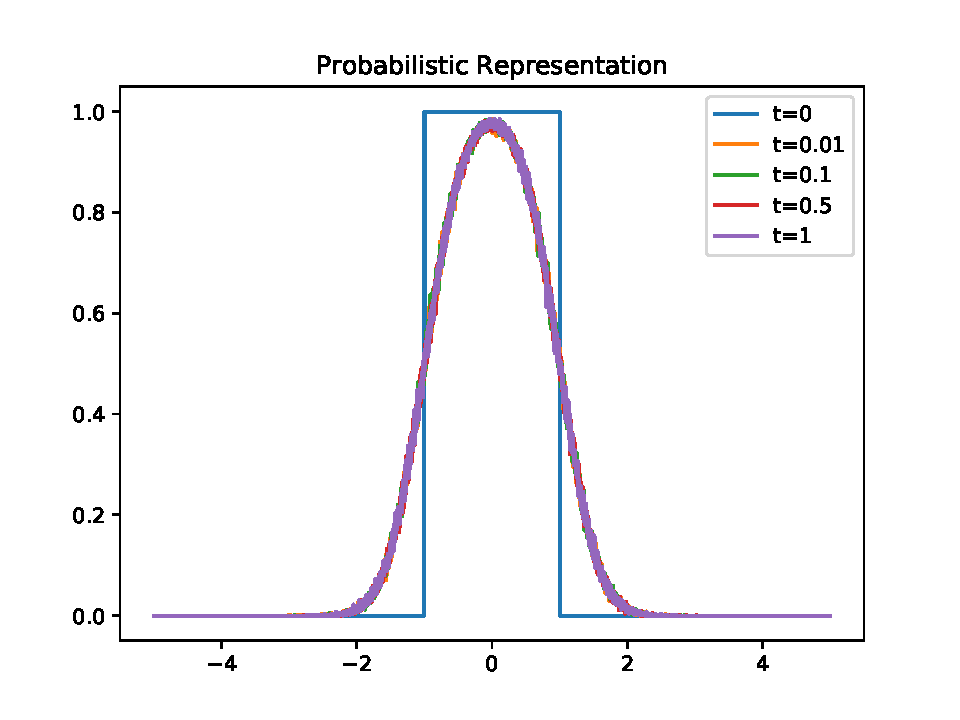
\includegraphics[width=\textwidth]{prob-sol}
            \caption{Numerical Solution by Monte Carlo Simulation}
            \label{fig:prob sol}
        \end{figure}
    \end{subproblem}

    \problem
    Denote $X_t$ driven by $\diff X_t=\mu(t,W_t)\diff t+\sigma(t,W_t)\diff W_t$
    with initial value $X_0=x$
    is the corresponded It\^o process. Then we have from It\^o's lemma
    that
    \[\diff f(X_t)=f'(X_t)\diff X_t+f''(X_t)\frac{1}{2}(\diff X_t)^2
    =\left(\mu f'+\frac{1}{2}\sigma f''\right)\diff t+\sigma f'\diff W_t\]
    which gives us
    \[f(X_t)=f(X_0)+\int_0^t\left(\mu f'+\frac{1}{2}\sigma f''\right)\diff s
    +\int_0^t\sigma f'\diff W_s\]
    Taking expectation on BHS yields
    \[E[f(X_t)]=f(x)+\int_0^tE\left[\mu f'+\frac{1}{2}\sigma f''\right]\diff s\]
    Therefore,
    \[Af(x)=\lim_{t\to 0^+}\frac{E[f(X_t)]-f(x)}{t}
    =E\left[\mu f'+\frac{1}{2}\sigma f''\right]\]
    % TODO Something wrong, definition of infinitestimal generator?


    \appendix
    \section{Python Code}
    \lstinputlisting[language=Python]{montecarlo.py}
\end{document}